\documentclass[11pt,a4paper,oneside]{report}             % Single-side
%\documentclass[11pt,a4paper,twoside,openright]{report}  % Duplex

%\PassOptionsToPackage{chapternumber=Huordinal}{magyar.ldf}
\usepackage{t1enc}
\usepackage[latin2]{inputenc}
\usepackage{amsmath}
\usepackage{amssymb}
\usepackage{enumerate}
\usepackage[thmmarks]{ntheorem}
\usepackage{graphics}
\usepackage{epsfig}
\usepackage{listings}
\usepackage{color}
%\usepackage{fancyhdr}
\usepackage{lastpage}
\usepackage{anysize}
\usepackage[magyar]{babel}
\usepackage{sectsty}
\usepackage{setspace}  % Ettol a tablazatok, abrak, labjegyzetek maradnak 1-es sorkozzel!
\usepackage[hang]{caption}
\usepackage{hyperref}

%--------------------------------------------------------------------------------------
% Main variables
%--------------------------------------------------------------------------------------
\newcommand{\vikszerzo}{B�dis-Szomor� Andr�s}
\newcommand{\vikkonzulens}{dr.~Konzulens Elem�r}
\newcommand{\vikcim}{Elektronikus terel�k}
\newcommand{\viktanszek}{M�r�stechnika �s Inform�ci�s Rendszerek Tansz�k}
\newcommand{\vikdoktipus}{Diplomaterv}
\newcommand{\vikdepartmentr}{B�dis-Szomor� Andr�s}

%--------------------------------------------------------------------------------------
% Page layout setup
%--------------------------------------------------------------------------------------
% we need to redefine the pagestyle plain
% another possibility is to use the body of this command without \fancypagestyle
% and use \pagestyle{fancy} but in that case the special pages
% (like the ToC, the References, and the Chapter pages)remain in plane style

\pagestyle{plain}
%\setlength{\parindent}{0pt} % �ttekinthet�bb, angol nyelv� dokumentumokban jellemz�
%\setlength{\parskip}{8pt plus 3pt minus 3pt} % �ttekinthet�bb, angol nyelv� dokumentumokban jellemz�
\setlength{\parindent}{12pt} % magyar nyelv� dokumentumokban jellemz�
\setlength{\parskip}{0pt}    % magyar nyelv� dokumentumokban jellemz�

\marginsize{35mm}{25mm}{15mm}{15mm} % anysize package
\setcounter{secnumdepth}{0}
\sectionfont{\large\upshape\bfseries}
\setcounter{secnumdepth}{2}
\singlespacing
\frenchspacing

%--------------------------------------------------------------------------------------
%	Setup hyperref package
%--------------------------------------------------------------------------------------
\hypersetup{
    bookmarks=true,            % show bookmarks bar?
    unicode=false,             % non-Latin characters in Acrobat�s bookmarks
    pdftitle={\vikcim},        % title
    pdfauthor={\vikszerzo},    % author
    pdfsubject={\vikdoktipus}, % subject of the document
    pdfcreator={\vikszerzo},   % creator of the document
    pdfproducer={Producer},    % producer of the document
    pdfkeywords={keywords},    % list of keywords
    pdfnewwindow=true,         % links in new window
    colorlinks=true,           % false: boxed links; true: colored links
    linkcolor=black,           % color of internal links
    citecolor=black,           % color of links to bibliography
    filecolor=black,           % color of file links
    urlcolor=black             % color of external links
}

%--------------------------------------------------------------------------------------
% Set up listings
%--------------------------------------------------------------------------------------
\lstset{
	basicstyle=\scriptsize\ttfamily, % print whole listing small
	keywordstyle=\color{black}\bfseries\underbar, % underlined bold black keywords
	identifierstyle=, 					% nothing happens
	commentstyle=\color{white}, % white comments
	stringstyle=\scriptsize\sffamily, 			% typewriter type for strings
	showstringspaces=false,     % no special string spaces
	aboveskip=3pt,
	belowskip=3pt,
	columns=fixed,
	backgroundcolor=\color{lightgray},
} 		
\def\lstlistingname{lista}	

%--------------------------------------------------------------------------------------
%	Some new commands and declarations
%--------------------------------------------------------------------------------------
\newcommand{\code}[1]{{\upshape\ttfamily\scriptsize\indent #1}}

% define references
\newcommand{\figref}[1]{\ref{fig:#1}.}
\renewcommand{\eqref}[1]{(\ref{eq:#1})}
\newcommand{\listref}[1]{\ref{listing:#1}.}
\newcommand{\sectref}[1]{\ref{sect:#1}}
\newcommand{\tabref}[1]{\ref{tab:#1}.}

\DeclareMathOperator*{\argmax}{arg\,max}
%\DeclareMathOperator*[1]{\floor}{arg\,max}
\DeclareMathOperator{\sign}{sgn}
\DeclareMathOperator{\rot}{rot}
\definecolor{lightgray}{rgb}{0.95,0.95,0.95}

\author{\vikszerzo}
\title{\viktitle}
\includeonly{
	guideline,%
	project,%
	titlepage,%
	declaration,%
	abstract,%
	introduction,%
	chapter1,%
	chapter2,%
	chapter3,%
	acknowledgement,%
	appendices,%
}
%--------------------------------------------------------------------------------------
%	Setup captions
%--------------------------------------------------------------------------------------
\captionsetup[figure]{
%labelsep=none,
%font={footnotesize,it},
%justification=justified,
width=.75\textwidth,
aboveskip=10pt}

\renewcommand{\captionlabelfont}{\small\bf}
\renewcommand{\captionfont}{\footnotesize\it}

%--------------------------------------------------------------------------------------
% Table of contents and the main text
%--------------------------------------------------------------------------------------
\begin{document}
\singlespacing
%--------------------------------------------------------------------------------------
% Rovid formai es tartalmi tajekoztato
%--------------------------------------------------------------------------------------

\footnotesize
\begin{center}
\large
\textbf{\Large �ltal�nos inform�ci�k, a diplomaterv szerkezete}\\
\end{center}

A diplomaterv szerkezete a BME Villamosm�rn�ki �s Informatikai Kar�n:
\begin{enumerate}
\item	Diplomaterv feladatki�r�s
\item	C�moldal
\item	Tartalomjegyz�k
\item	A diplomatervez� nyilatkozata az �n�ll� munk�r�l �s az elektronikus adatok kezel�s�r�l
\item	Tartalmi �sszefoglal� magyarul �s angolul
\item	Bevezet�s: a feladat �rtelmez�se, a tervez�s c�lja, a feladat indokolts�ga, a diplomaterv fel�p�t�s�nek r�vid �sszefoglal�sa
\item	A feladatki�r�s pontos�t�sa �s r�szletes elemz�se
\item	El�zm�nyek (irodalomkutat�s, hasonl� alkot�sok), az ezekb�l levonhat� k�vetkeztet�sek
\item	A tervez�s r�szletes le�r�sa, a d�nt�si lehet�s�gek �rt�kel�se �s a v�lasztott megold�sok indokl�sa
\item	A megtervezett m�szaki alkot�s �rt�kel�se, kritikai elemz�se, tov�bbfejleszt�si lehet�s�gek
\item	Esetleges k�sz�netnyilv�n�t�sok
\item	R�szletes �s pontos irodalomjegyz�k
\item	F�ggel�k(ek)
\end{enumerate}

Felhaszn�lhat� a k�vetkez� oldalt�l kezd�d� \LaTeX-Diplomaterv sablon dokumentum tartalma. 

A diplomaterv szabv�nyos m�ret� A4-es lapokra ker�lj�n. Az oldalak t�k�rmarg�val k�sz�ljenek (mindenhol 2.5cm, baloldalon 1cm-es k�t�ssel). Az alap�rtelmezett bet�k�szlet a 12 pontos Times New Roman, m�sfeles sork�zzel.

Minden oldalon - az els� n�gy szerkezeti elem kiv�tel�vel - szerepelnie kell az oldalsz�mnak.

A fejezeteket decim�lis beoszt�ssal kell ell�tni. Az �br�kat a megfelel� helyre be kell illeszteni, fejezetenk�nt decim�lis sz�mmal �s kifejez� c�mmel kell ell�tni. A fejezeteket decim�lis al�oszt�ssal sz�mozzuk, maxim�lisan 3 al�oszt�s m�lys�gben (pl. 2.3.4.1.). Az �br�kat, t�bl�zatokat �s k�pleteket c�lszer� fejezetenk�nt k�l�n sz�mozni (pl. 2.4. �bra, 4.2 t�bl�zat vagy k�pletn�l (3.2)). A fejezetc�meket igaz�tsuk balra, a norm�l sz�vegn�l viszont haszn�ljunk sorkiegyenl�t�st. Az �br�kat, t�bl�zatokat �s a hozz�juk tartoz� c�met igaz�tsuk k�z�pre. A c�m a jel�lt r�sz alatt helyezkedjen el.

A k�peket lehet�leg rajzol� programmal k�sz�ts�k el, az egyenleteket egyenlet-szerkeszt� seg�ts�g�vel �rj�k le (A \LaTeX~ehhez k�zenfekv� megold�sokat ny�jt).

Az irodalomjegyz�k sz�vegk�zi hivatkoz�sa t�rt�nhet a Harvard-rendszerben (a szerz� �s az �vsz�m megad�s�val) vagy sorsz�mozva. A teljes lista n�vsor szerinti sorrendben a sz�veg v�g�n szerepeljen (sorsz�mozott irodalmi hivatkoz�sok eset�n hivatkoz�si sorrendben). A szakirodalmi forr�sok c�meit azonban mindig az eredeti nyelven kell megadni, esetleg z�r�jelben a ford�t�ssal. A list�ban szerepl� valamennyi publik�ci�ra hivatkozni kell a sz�vegben (a \LaTeX-sablon a Bib\TeX~seg�ts�g�vel mindezt automatikusan kezeli). Minden publik�ci� a szerz�k ut�n a k�vetkez� adatok szerepelnek: foly�irat cikkekn�l a pontos c�m, a foly�irat c�me, �vfolyam, sz�m, oldalsz�m t�l-ig. A foly�irat c�meket csak akkor r�vid�ts�k, ha azok nagyon k�zismertek vagy nagyon hossz�ak. Internet hivatkoz�sok megad�sakor fontos, hogy az el�r�si �t el�tt megadjuk az oldal tulajdonos�t �s tartalm�t (mivel a link egy id� ut�n ak�r el�rhetetlenn� is v�lhat), valamint az el�r�s id�pontj�t.

\vspace{5mm}
Fontos:
\begin{itemize}
	\item A szakdolgozat k�sz�t� / diplomatervez� nyilatkozata (a jelen sablonban szerepl� sz�vegtartalommal) k�telez� el��r�s Karunkon ennek hi�ny�ban a szakdolgozat/diplomaterv nem b�r�lhat� �s nem v�dhet� !
	\item Mind a dolgozat, mind a mell�klet maxim�lisan 15 MB m�ret� lehet !
\end{itemize}

\vspace{5mm}
\begin{center}
J� munk�t, sikeres szakdolgozat k�sz�t�st ill. diplomatervez�st k�v�nunk !
\end{center}

\normalsize

%--------------------------------------------------------------------------------------
% Feladatkiiras (a tanszeken atveheto, kinyomtatott valtozat)
%--------------------------------------------------------------------------------------
\clearpage
\begin{center}
\large
\textbf{FELADATKI�R�S}\\
\end{center}

A feladatki�r�st a tansz�ki adminisztr�ci�ban lehet �tvenni, �s a leadott munk�ba eredeti, tansz�ki pecs�ttel ell�tott �s a tansz�kvezet� �ltal al��rt lapot kell belef�zni (ezen oldal \emph{helyett}, ez az oldal csak �tmutat�s). Az elektronikusan felt�lt�tt dolgozatban m�r nem kell beleszerkeszteni ezt a feladatki�r�st.





\pagenumbering{arabic}
\onehalfspacing
%--------------------------------------------------------------------------------------
%	The title page
%--------------------------------------------------------------------------------------
\begin{titlepage}
\begin{center}

\includegraphics[width=60mm,keepaspectratio]{figures/BMElogo.png}\\
\vspace{0.3cm}
\textbf{Budapesti M�szaki �s Gazdas�gtudom�nyi Egyetem}\\
\textmd{Villamosm�rn�ki �s Informatikai Kar}\\
\textmd{\viktanszek}\\[5cm]

\vspace{0.4cm}
{\huge \bfseries \vikcim}\\[0.8cm]
\vspace{0.5cm}
\textsc{\Large \vikdoktipus}\\[4cm]

\begin{tabular}{cc}
 \makebox[7cm]{\emph{K�sz�tette}} & \makebox[7cm]{\emph{Konzulens}} \\
 \makebox[7cm]{\vikszerzo} & \makebox[7cm]{\vikkonzulens}
\end{tabular}

\vfill
{\large \today}
\end{center}
\end{titlepage}



\tableofcontents\vfill
%--------------------------------------------------------------------------------------
% Nyilatkozat
%--------------------------------------------------------------------------------------
\begin{center}
\large
\textbf{HALLGAT�I NYILATKOZAT}\\
\end{center}

Alul�rott \emph{\vikszerzo}, szigorl� hallgat� kijelentem, hogy ezt a szakdolgozatot/ diplomatervet \textcolor{blue}{(nem k�v�nt t�rlend�)} meg nem engedett seg�ts�g n�lk�l, saj�t magam k�sz�tettem, csak a megadott forr�sokat (szakirodalom, eszk�z�k stb.) haszn�ltam fel. Minden olyan r�szt, melyet sz� szerint, vagy azonos �rtelemben, de �tfogalmazva m�s forr�sb�l �tvettem, egy�rtelm�en, a forr�s megad�s�val megjel�ltem.

Hozz�j�rulok, hogy a jelen munk�m alapadatait (szerz�(k), c�m, angol �s magyar nyelv� tartalmi kivonat, k�sz�t�s �ve, konzulens(ek) neve) a BME VIK nyilv�nosan hozz�f�rhet� elektronikus form�ban, a munka teljes sz�veg�t pedig az egyetem bels� h�l�zat�n kereszt�l (vagy autentik�lt felhaszn�l�k sz�m�ra) k�zz�tegye. Kijelentem, hogy a beny�jtott munka �s annak elektronikus verzi�ja megegyezik. D�k�ni enged�llyel titkos�tott diplomatervek eset�n a dolgozat sz�vege csak 3 �v eltelte ut�n v�lik hozz�f�rhet�v�.

\begin{flushleft}
\vspace*{1cm}
Budapest, \today
\end{flushleft}

\begin{flushright}
 \vspace*{1cm}
 \makebox[7cm]{\rule{6cm}{.4pt}}\\
 \makebox[7cm]{\emph{\vikszerzo}}\\
 \makebox[7cm]{hallgat�}
\end{flushright}
\thispagestyle{empty}

\vfill
\clearpage
\thispagestyle{empty} % an empty page


%----------------------------------------------------------------------------
% Abstract in hungarian
%----------------------------------------------------------------------------
\chapter*{Kivonat}\addcontentsline{toc}{chapter}{Kivonat}

Jelen dokumentum egy diplomaterv sablon, amely formai keretet ad a BME Villamosm�rn�ki �s Informatikai Kar�n v�gz� hallgat�k �ltal elk�sz�tend� szakdolgozatnak �s diplomatervnek. A sablon haszn�lata opcion�lis. Ez a sablon \LaTeX~alap�, a \emph{TeXLive} \TeX-implement�ci�val �s a PDF-\LaTeX~ford�t�val m�k�d�k�pes.
\vfill

%----------------------------------------------------------------------------
% Abstract in english
%----------------------------------------------------------------------------
\chapter*{Abstract}\addcontentsline{toc}{chapter}{Abstract}

This document is a \LaTeX-based skeleton for BSc/MSc~theses of students at the Electrical Engineering and Informatics Faculty, Budapest University of Technology and Economics. The usage of this skeleton is optional. It has been tested with the \emph{TeXLive} \TeX~implementation, and it requires the PDF-\LaTeX~compiler.
\vfill


%----------------------------------------------------------------------------
\chapter*{Bevezet�}\addcontentsline{toc}{chapter}{Bevezet�}
%----------------------------------------------------------------------------

A bevezet� tartalmazza a diplomaterv-ki�r�s elemz�s�t, t�rt�nelmi el�zm�nyeit, a feladat indokolts�g�t (a motiv�ci� le�r�s�t), az eddigi megold�sokat, �s ennek t�kr�ben a hallgat� megold�s�nak �sszefoglal�s�t.

A bevezet� szok�s szerint a diplomaterv fel�p�t�s�vel z�r�dik, azaz annak r�vid le�r�s�val, hogy melyik fejezet mivel foglalkozik.


%----------------------------------------------------------------------------
\chapter{\LaTeX-eszk�z�k}\label{sect:LatexTools}
%----------------------------------------------------------------------------
\section{A szerkeszt�shez haszn�latos, Windows alap� eszk�z�k}
%----------------------------------------------------------------------------
Ez a sablon Windows oper�ci�s rendszer alatt k�sz�lt TeXnicCenter 1 Beta 7.01 szerkeszt�vel. A TeXnicCenter egy \LaTeX-szerkeszt�program sz�mtalan hasznos -- �s r�ad�sul j�l m�k�d� -- szolg�ltat�ssal (\figref{TexnicCenter} �bra). A szoftver ingyenesen let�lthet� a\\\url{http://www.texniccenter.org/} c�mr�l.

\begin{figure}[!ht]
\centering
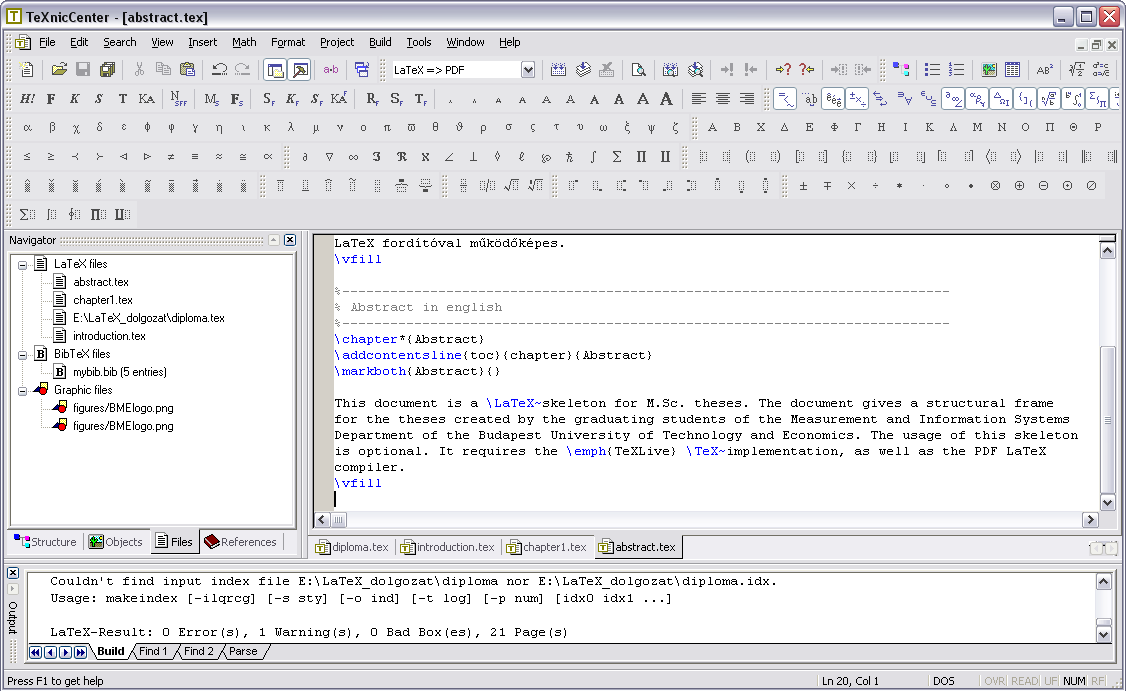
\includegraphics[width=150mm, keepaspectratio]{figures/TeXnicCenter.png}
\caption{A TeXnicCenter Windows alap� \LaTeX-szerkeszt�.} 
\label{fig:TexnicCenter}
\end{figure}

Egy m�sik haszn�lhat� Windows alap� szerkeszt�program a LEd (LaTeX Editor,\\\url{http://www.latexeditor.org/}), a TeXnicCenter azonban stabilabb, gyorsabb, �s jobban haszn�lhat�.

%----------------------------------------------------------------------------
\section{A dokumentum leford�t�sa Windows alatt}
%----------------------------------------------------------------------------
A TeXnicCenter �s a LEd kiz�r�lag szerkeszt�program (b�r az ut�bbiban DVI-n�zeget� is van), �gy a dokumentum ford�t�s�hoz sz�ks�ges eszk�z�ket nem tartalmazza. Windows alatt alapvet�en k�t lehet�s�g k�z�l �rdemes v�lasztani: MiKTeX (\url{http://miktex.org/}) �s TeXLive (\url{http://www.tug.org/texlive/}) programcsomag. Az ut�bbi m�k�dik Mac OS X, GNU/Linux alatt �s Unix-sz�rmaz�kokon is. A MiKTeX egy alapcsomag telep�t�se ut�n mindig let�lti a haszn�lt funkci�khoz sz�ks�ges, de lok�lisan hi�nyz� \TeX-csomagokat, m�g a TeXLive DVD ISO verz�ban f�rhet� hozz�. Ez a dokumentum TeXLive 2008 programcsomag seg�ts�g�vel fordult, amelynek DVD ISO verzi�ja a megadott oldalr�l let�lthet�. A sablon leford�t�s�hoz a disztrib�ci�ban szerepl� \verb+magyar.ldf+ f�jlt a \verb+http://www.math.bme.hu/latex/+ v�ltozatra kell cser�lni, vagy az ut�bbi v�ltozatot be kell m�solni a projekt-k�nyvt�rba (ahogy ezt meg is tett�k a sablonban) k�l�nben anom�li�k tapasztalhat�k a dokumentumban (pl. az �bra- �s t�bl�zat-al��r�sok form�tuma nem a be�ll�tott lesz, vagy bizonyos oldalakon megjelenik alap�telmez�sben egy fejl�c). A TeXLive 2008-at m�g nem kell k�l�n telep�teni a g�pre, elegend� DVD-r�l (vagy az ISO f�jlb�l k�zvetlen�l, pl. DaemonTools-szal) haszn�lni. 

A \TeX-eszk�z�ket tartalmaz� programcsomag bin�risainak el�r�si �tj�t minden esetben be kell �ll�tani a szerkeszt�programban, p�ld�ul TeXnicCenter eset�n legegyszer�bben a \verb+Build / Define output profiles...+ men�ponttal el�h�vott dial�gusablakban a \verb+Wizard...+ gombra kattintva tehetj�k ezt meg.

A PDF-\LaTeX~haszn�lata eset�n a gener�lt dokumentum k�zvetlen�l PDF-form�tumban �ll rendelkez�sre. Amennyiben a PDF-f�jl egy PDF-n�z�ben (pl. Adobe Acrobat Reader vagy Foxit PDF Reader) meg van nyitva, akkor a f�jlle�r�t a PDF-n�z� program tipikusan lefoglalja. Ilyen esetben a dokumentum �jraford�t�sa hiba�zenettel kil�p. Ha bez�rjuk �s �jra megnyitjuk a PDF dokumentumot, akkor pedig a PDF-n�z�k t�bbs�ge az els� oldalon nyitja meg a dokumentumot, nem a legut�bb olvasott oldalon. Ezzel szemben p�ld�ul az egyszer� �s ingyenes \textcolor{blue}{Sumatra PDF} nev� program k�pes arra, hogy a megnyitott dokumentum megv�ltoz�s�t detekt�lja, �s friss�tse a n�zetet az aktu�lis oldal megtart�s�val.

%----------------------------------------------------------------------------
\section{Eszk�z�k Linuxhoz}
%----------------------------------------------------------------------------
Linux oper�ci�s rendszer alatt is rengeteg szerkeszt�program van, pl. a KDE alap� Kile j�l haszn�lhat�. Ez ingyenesen let�lthet�, vagy �ppens�ggel az adott Linux-disztrib�ci� eleve tartalmazza, ahogyan a dokumentum ford�t�s�hoz sz�ks�ges csomagokat is. Az Ubuntu Linux disztrib�ci�k alatt p�ld�ul legt�bbsz�r a \verb+texlive-base+ csomag telep�t�s�vel haszn�lhat�k a \LaTeX-eszk�z�k.


\setcounter{chapter}{2}
%----------------------------------------------------------------------------
\chapter*{2. Tétel}
%----------------------------------------------------------------------------

\textbf{Témakörök:} A lineáris programozás alapfeladata, kétváltozós feladat grafikus megoldása. Lineáris egyenlőtlenség-rendszer megoldása Fourier-Motzkin eliminációval.

\noindent\hrulefill

\section*{LP feladatok alakjai}

\begin{theo} TODO \end{theo}

\section*{Dualitás tétel}

\begin{theo} 
Ha a $max \lbrace c x: Ax\leq b\rbrace$ primál program megoldható és felülről korlátos:
\begin{enumerate}
\item	a $min \lbrace yb: yA=c,y\geq 0\rbrace$ duális program is megoldható és alulról korlátos,
\item	a primál programnak létezik maximuma és a duális programnak létezik minimuma,
\item	továbbá ezek megegyeznek: $max\lbrace cx: Ax\leq b\rbrace = min\lbrace yb: yA=c,y\geq 0\rbrace$
\end{enumerate}
\end{theo}
Megjegyzés: $(2)$-re szükség van, mert egy számhalmaz felülről korlátosságából általában nem következik, hogy létezik maximuma.

\section*{Ekvivalens alak}
\begin{theo}
Ha a $max\lbrace cx:AX\leq b,x\geq 0\rbrace$ primál program megoldható és felülről korlátos:
\begin{enumerate}
\item a $min \lbrace yb:yA\geq c, y \geq 0\rbrace$ duális program is megoldható és alulról korlátos,
\item	a primál programnak létezik maximuma és a duális programnak létezik minimuma,
\item	továbbá ezek megegyeznek: $max\lbrace cx:AX\leq b,x\geq 0\rbrace = min \lbrace yb:yA\geq c, y \geq 0\rbrace$
\end{enumerate}
\end{theo}

\newpage

\section*{Bonyolultság}
\subsection*{LP feladat, eldöntési problémaként megfogalmazva}
Van-e az $Ax\leq b$ feltételt kielégítő $x$ vektorok között olyan, amelyre $cx\geq t$?
\begin{itemize}
	\item NP-beli: tanú egy ilyen $x$
	\item co-NP-beli: ha $cx<t$, akkor a duális megoldása ($y$) tanú erre
	\item (a tanúk polinomiális méretűek)
\end{itemize}

\subsection*{Módszerek}
\begin{itemize}
\item Szimplex módszer (1947, Dantzig): nem polinomiális, de a gyakorlati alkalmazások során gyors
\item Ellipszoid módszer (1979, Hacsijan): polinomiális, de a gyakorlati alkalmazások során lassú
\item Belső pontos módszerek (1984, Karmarkar): polinomiális, a gyakorlati alkalmazások során eredményes, de nem elterjedt
\end{itemize}


\setcounter{chapter}{3}
%----------------------------------------------------------------------------
\chapter*{3. Tétel}
%----------------------------------------------------------------------------

\textbf{Témakörök:} Farkas-lemma (két alakban). A lineáris program célfüggvénye felülről korlátosságának feltételei.

\noindent\hrulefill

\section*{Farkas-lemma 1.}
Tetszőleges $A$, $b$ esetén az alábbi rendszerek közül pontosan az egyiknek van megoldása:
\begin{itemize}
\item (1) $Ax\leq b$
\item (2) $yA=0$, $y\geq 0$, $yb<0$
\end{itemize}

\section*{Farkas-lemma 2.}
Tetszőleges $A$, $b$ esetén az alábbi rendszerek közül pontosan az egyiknek van megoldása:
\begin{itemize}
\item (1) $Ax=b$, $x\geq 0$
\item (2) $yA\geq 0$, $yb<0$
\end{itemize}

\textbf{Megjegyzés:} a tétel (1) állítása felfogható egyenlőtlenség rendszerként is: $Ax\leq b$, $(-A)x\leq (-b)$, $(-E)x\leq 0$. Erre is alkalmazható a Farkas-lemma 1. alakja.

\section*{Következmény}
Tetszőleges $A$, $b$ esetén az alábbi rendszerek közül pontosan az egyiknek van megoldása:
\begin{itemize}
\item (1) $Ax=b$
\item (2) $yA=0$, $yb\neq 0$
\end{itemize}

\section*{Célfüggvény korlátossága}
Tegyük fel, hogy $Ax\leq b$ megoldható, $c$ tetszőleges adott vektor. Ekkor az alábbi állítások ekvivalensek:
\begin{itemize}
\item (1) az $Ax\leq b$ megoldáshalmazán $cx$ felülről korlátos,
\item (2) nincs megoldása az $Az\leq 0$, $cz>0$ rendszernek,
\item (3) van megoldása az $yA=c$, $y\geq 0$ rendszernek.
\end{itemize}
%----------------------------------------------------------------------------
\chapter*{K�sz�netnyilv�n�t�s}\addcontentsline{toc}{chapter}{K�sz�netnyilv�n�t�s}
%----------------------------------------------------------------------------

Ez nem k�telez�, ak�r t�r�lhet� is. Ha a szerz� sz�ks�g�t �rzi, itt lehet k�sz�netet nyilv�n�tani azoknak, akik hozz�j�rultak munk�jukkal ahhoz, hogy a hallgat� a szakdolgozatban vagy diplomamunk�ban le�rt feladatokat sikeresen elv�gezze. A konzulensnek val� k�sz�netnyilv�n�t�s sem k�telez�, a konzulensnek hivatalosan is dolga, hogy a hallgat�t konzult�lja.

%\listoffigures\addcontentsline{toc}{chapter}{�br�k jegyz�ke}
%\listoftables\addcontentsline{toc}{chapter}{T�bl�zatok jegyz�ke}

\bibliography{mybib}
\addcontentsline{toc}{chapter}{Irodalomjegyz�k}
\bibliographystyle{plain}

%----------------------------------------------------------------------------
\appendix
%----------------------------------------------------------------------------
\chapter*{F�ggel�k}\addcontentsline{toc}{chapter}{F�ggel�k}
\setcounter{chapter}{6}  % a fofejezet-szamlalo az angol ABC 6. betuje (F) lesz
\setcounter{equation}{0} % a fofejezet-szamlalo az angol ABC 6. betuje (F) lesz
\numberwithin{equation}{section}
\numberwithin{figure}{section}
\numberwithin{lstlisting}{section}
%\numberwithin{tabular}{section}

%----------------------------------------------------------------------------
\section{A TeXnicCenter fel�lete}
%----------------------------------------------------------------------------
\begin{figure}[!ht]
\centering
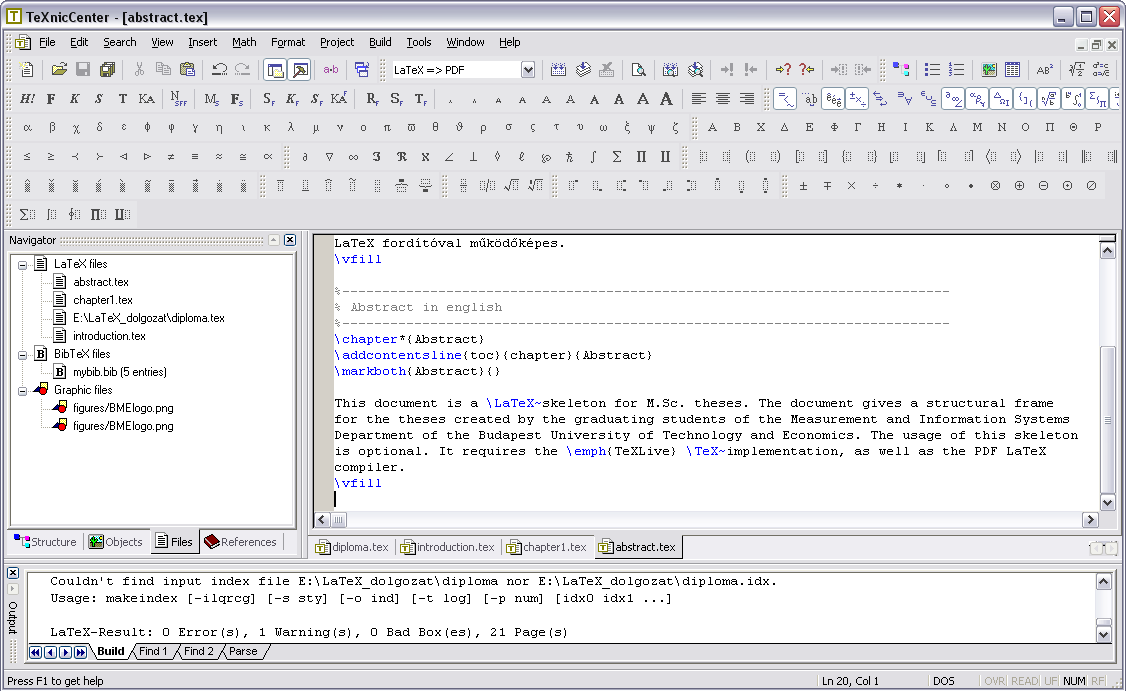
\includegraphics[width=150mm, keepaspectratio]{figures/TeXnicCenter.png}
\caption{A TeXnicCenter Windows alap� \LaTeX-szerkeszt�.} 
\end{figure}

%----------------------------------------------------------------------------
\clearpage\section{V�lasz az ,,�let, a vil�gmindens�g, meg minden'' k�rd�s�re}
%----------------------------------------------------------------------------
A Pitagorasz-t�telb�l levezetve
\begin{align}
c^2=a^2+b^2=42.
\end{align}
A Faraday-indukci�s t�rv�nyb�l levezetve
\begin{align}
\rot E=-\frac{dB}{dt}\hspace{1cm}\longrightarrow \hspace{1cm}
U_i=\oint\limits_\mathbf{L}{\mathbf{E}\mathbf{dl}}=-\frac{d}{dt}\int\limits_A{\mathbf{B}\mathbf{da}}=42.
\end{align}







\label{page:last}
\end{document}
